\documentclass[11pt]{article}
\usepackage[left=20mm, right=20mm, top=20mm, bottom=20mm]{geometry} %this sets the page margins 
\usepackage{amsmath}
\usepackage{amsfonts}
\usepackage{amssymb}
\usepackage{graphicx}
\usepackage{wrapfig}
\usepackage{subcaption}
\usepackage[justification=centering]{caption}
\usepackage{setspace}
\doublespacing
\setlength{\parindent}{1cm}
\usepackage{color}
\usepackage{framed}
\usepackage{comment}
\usepackage{pdfpages}
\usepackage{courier}
\usepackage{float}
\usepackage{helvet}
\renewcommand{\familydefault}{\sfdefault}
\usepackage[hyphens]{url}
\usepackage{listings,xcolor}
\usepackage[numbered,framed]{matlab-prettifier}
\renewcommand{\lstlistingname}{Codebox}% Listing -> Codebox

\newcommand\undermat[2]{%
  \makebox[0pt][l]{$\smash{\underbrace{\phantom{%
    \begin{matrix}#2\end{matrix}}}_{\text{$#1$}}}$}#2}

\numberwithin{equation}{subsection}
\usepackage{titlesec}
\newcommand{\sectionbreak}{\clearpage}
\DeclareMathOperator\arctanh{arctanh}

%% THIS BIT MAKES CLICKABLE PDF LINKS
\usepackage{hyperref}
\hypersetup{
    colorlinks,
    citecolor=black,
    filecolor=black,
    linkcolor=black,
    urlcolor=black
}
%%


\author{Henry Fletcher}

\title{Making Flash Memory Work}

%%%%%%%%%%%%%%%%%%%%%%%%%%%%%%%%%%%%%%%%%%%%%%%%%%%%%%%%%%%%%%%%%%%%%%%%%%%%
\begin{document}

\section{Executive Summary}

Modern flash memory is reliant on error-correcting code to ensure error-free operation. Current flash memory architectures often use linear block codes for this purpose (e.g. Reed-Solomon, Hamming or BCH codes). However, the recent rediscovery of LDPC (Low Density Parity Check) codes, which can achieve superior performance close to the Shannon Limit, has generated much interest in the NAND memory industry. These codes could be used to further improve error correction capability in flash memory, thus allowing for more densely packed memory cells and thus larger capacity drives.

The general aim of this project is to produce a MATLAB simulation of how an error correction system using LDPC codes would work for flash memory.  By combining both an error generation and an error correction model, it will be possible to benchmark these rediscovered codes, and subsequently compare them to current generation technologies.

\tableofcontents

\section{Introduction}

\section{Overview of Linear Block Codes}

Linear block codes are one of the two main classes of forward error correction (FEC), with the other main type being convolutional coding. A linear block code essentially takes a block of binary data, and adds additional redundant data onto it. This block can then be transmitted over a noisy channel, and subsequently decoded at the receiver. The redundant bits in the block are used as parity check equations, which allows a linear block code to both detect and correct errors. 

\subsection{Definitions for Linear Block Codes} \label{3.1:definitions}
All linear block codes can be described using a set of standard terms and symbols. For this project, all codes use a binary alphabet of $\{0,1\}$ and hence all operations are over this binary field. $n$ is the block length, the total size of the output codeword. $k$ is the message length, the size of the information vector prior to encoding. An $(n,k)$ error correcting \textit{code} $\mathcal{C}$, will produce a set of $2^k$ output \textit{codewords} $\mathbf{c}$. Hence, $\mathbf{c} \in \mathcal{C}$. 

The rate of any linear block code, $R$, is defined as: 
\begin{equation}
R = \dfrac{k}{n}
\end{equation}
The rate is a measure of the number of information bits compared to the total number of transmitted codeword bits. A high rate code will be more efficient in terms of useful information transmitted, but will have a poorer error correction capability. In Flash Memory, very high rate ($R > 0.9$) codes are used in order to maximise the amount of usable storage space. Conversely, an example use of low rate codes would be in deep-space probe transmissions, where receiving error-free data is more important than rate of transmission.

A linear block code can be represented in two ways: through the $k \times n$ generator matrix $\mathbf{G}$, or the $(n - k) \times n$ parity check matrix $\mathbf{H}$. Each is the null-space of the other, such that:
\begin{equation}
\mathbf{G H}^\top = 0
\end{equation}
Unsurprisingly, the generator matrix $\mathbf{G}$ is used in the transmission side when encoding data, and the parity check matrix $\mathbf{H}$ is used at the receiver to detect and correct any errors.

At the transmitter, if we take a $1 \times k$ input vector of binary data $\mathbf{x}$, the method of encoding this data into a codeword $\mathbf{c}$, is simply a multiplication operation:
\begin{equation}
\mathbf{c = xG}
\end{equation}
At the receiver, a similar operation is performed:
%%%% CHECK THAT THIS IS CORRECT !!! %%%%%
\begin{equation}
\mathbf{s = c H}^\top
\end{equation}
where $\mathbf{s}$ is known as the \textit{syndrome}. If the syndrome is the all zero vector, then error free transmission has occurred. Conversely, if any bit of the syndrome is 1, then this represents a particular error pattern. For small block lengths, these error pattern's can be pre-calculated and saved as a table, allowing for syndrome lookup decoding. The table identifies the exact location of a bit error in the codeword, which can then be `flipped' in order to perform error correction.

An example of a \textit{systematic} generator matrix, in this case a matrix known as the \textit{Hamming(7,4) code}, takes the form:
\begin{equation}
\mathbf{G} = 
\left(
\begin{array}{ccc|cccc}
  1 & 1 & 0 & 1 & 0 & 0 & 0 \\
  0 & 1 & 1 & 0 & 1 & 0 & 0 \\
  1 & 1 & 1 & 0 & 0 & 1 & 0 \\
  %1 & 0 & 1 & 0 & 0 & 0 & 1 \\
  \undermat{n-k}{1 & 0 & 1} & \undermat{k}{0 & 0 & 0 & 1} \\
  \end{array}
\right)
\end{equation}
\\
In this code, 4 information bits are encoded into 7 output bits.
Notice the identity matrix in the right portion of the generator matrix. This means that the 4 message ($k$) bits are always encoded at the end of the codeword, with the parity check ($n-k$) bits at the start of the codeword. This is why it is \textit{systematic}. At the decoder, it is then easy to extract the (uncorrected) message bits from the codeword, simply by looking at the last 4 bits.

\subsection{Hamming weight, distance, and error correction capability}

An important metric when discussing error correcting codes is the concept of the Hamming weight. 
For any codeword, the Hamming weight is defined as the total number of non-zero elements in a given codeword. 
Another metric, the minimum weight ($w_{min}$), is simply the minimum value from the set of all Hamming weight's for a given code, excluding the all-zero case.

\textbf{Example:}
A fictional example (6,2) code could have the following codewords:

\begin{center}
\begin{tabular}{ c | c | c }
Message (2 bits) & Codeword (6 bits) & Hamming weight \\
\hline
0 0 & 0 0 0 0 0 0 & 0 \\
0 1 & 1 0 1 0 1 0 & 3 \\
1 0 & 0 0 1 1 0 0 & 2 \\
1 1 & 1 0 0 1 1 0 & 3 \\
\end{tabular}
\end{center}
For this code, the minimum weight ($w_{min}$) is 2, since that is the smallest value of the Hamming weight's excluding the all-zero case.

Another metric used is the Hamming distance. The Hamming distance defines how `close' any two codewords are to each other. Codewords that are `far away' from each other are less likely to be decoded in error, and hence the Hamming distance determines how `good' a code is at error detection and correction. Formally, the Hamming distance is defined as the number of (binary) places that any 2 codewords differ. Analogous to the minimum weight, there is also a minimum distance ($d_{min}$), which is the minimum value from the set of all Hamming distances for a given code, excluding the trivial case of comparing a codeword to itself.

An important result arises because of the use of binary arithmetic, in that the minimum Hamming weight is in fact equal to the minimum Hamming distance:
\begin{equation}
d_{min} = w_{min}
\end{equation}

It is now possible to present the results that describe, for linear block codes, their error correction and detection performance:

\medskip
\noindent
\textbf{Error Detection Theorem:}
\textit{A linear block code with minimum weight $w_{min}$ is able to detect up to $e$ errors:}
\begin{equation}
e_{detectable} = w_{min} - 1
\end{equation}

\noindent
\textbf{Error Correction Theorem:}
\textit{A linear block code with minimum weight $w_{min}$ is able to correct up to $e$ errors:}
\begin{equation}
e_{correctable} = \dfrac{w_{min} - 1}{2}
\end{equation}

\subsection{Low Density Parity Check codes}
A particular class of codes, known as ``Low Density Parity Check" (LDPC) codes, are of particular interest and relevance to this project. LDPC codes are generally considered to be some of the best performing linear block codes available, in terms of error performance, with some codes getting within a fraction of the Shannon Limit. Additionally, LDPC codes have no patent and hence no licensing costs, making them attractive for real world use.(??!).

LDPC codes were originally discovered by R.G. Gallager in 1962. Then known as ``Gallager codes", they were defined by a sparse parity check matrix with low column weights. Gallager also worked on a probabilty based decoding method for these codes, which proved to have promising performance. However for various reasons, these codes were essentially lost in favour of other more practical codes. It is possible that the decoding complexity for LDPC was, at the time, too great for the computational power then available.\footnote{Personal opinion. Even today, decoding LDPC using near-optimum belief propagation on a PC is computationally expensive, whilst on dedicated ASIC hardware consumes large amounts of power.}

Modern LDPC codes were re-discovered by J.C. MacKay in 1996. MacKay demonstrated that LDPC codes could be decoded using probabilistic methods, even beyond the bound set by their minimum distance. Today, LDPC codes are seeing a resurgence in various applications. Most notably in the DVB-S2 standards for digital HD satellite broadcast, 10GBase-T Ethernet and as optional `add-ons' to the 802.11n/ac wi-fi standards.

Disadvantages of LDPC include the fact that there still exists a small (often in the region of $10^{-6}$ to $10^{-9}$) probability of error after decoding, known as the `error-floor'. This can be avoided by using a second high rate, `inner' Error Correcting Code such as BCH or Reed-Solomon to remove the last few bit errors. Other issues include decoding complexity. Whilst decoding time is linear with block length, decoding using the belief propagation algorithm is still problematic, especially for low power mobile devices. Most applications of LDPC so far have been on mains-powered equipment.


\textbf{Example:}
A specific DVB-S2 code, with $n = 64800$ and $r = 0.9$, has a total of $194,399$ non-zero elements in it's parity check matrix $\mathbf{H}$. However, the non-zero elements account for just 0.04\% of the total matrix: The vast majority of $\mathbf{H}$ is empty. It is therefore easy to see why they are called ``Low Density". In this project, this specific high-rate code is used extensively, especially when modelling the memory-specific case in section ?????????.

\subsection{Channel Capacity}

Channel capacity stuff to go here

\section{Overview of Flash Memory Technology} 

\section{Decoding of LDPC Codes}
Using syndrome lookup decoding as described in section \ref{3.1:definitions} would be nearly impossible for longer block lengths. There is a much better, iterative decoding method that can be used for any linear block code, and which is linear in block length. It is called the belief propagation algorithm (also known as the sum-product algorithm or the message passing algorithm). 

There are two distinct methods of belief propagation: Hard decision decoding and soft decision decoding. In hard decision decoding, the error correction algorithm only receives binary data (i.e. \{1,0\}). In soft decision decoding, the error correction algorithm receives a numerical likelihood of the data being either a 0 or 1. Soft decision decoding will therefore result in superior performance, since it is able to make use of the additional 'soft' information that is otherwise discarded.

\begin{figure}[h]
\centering
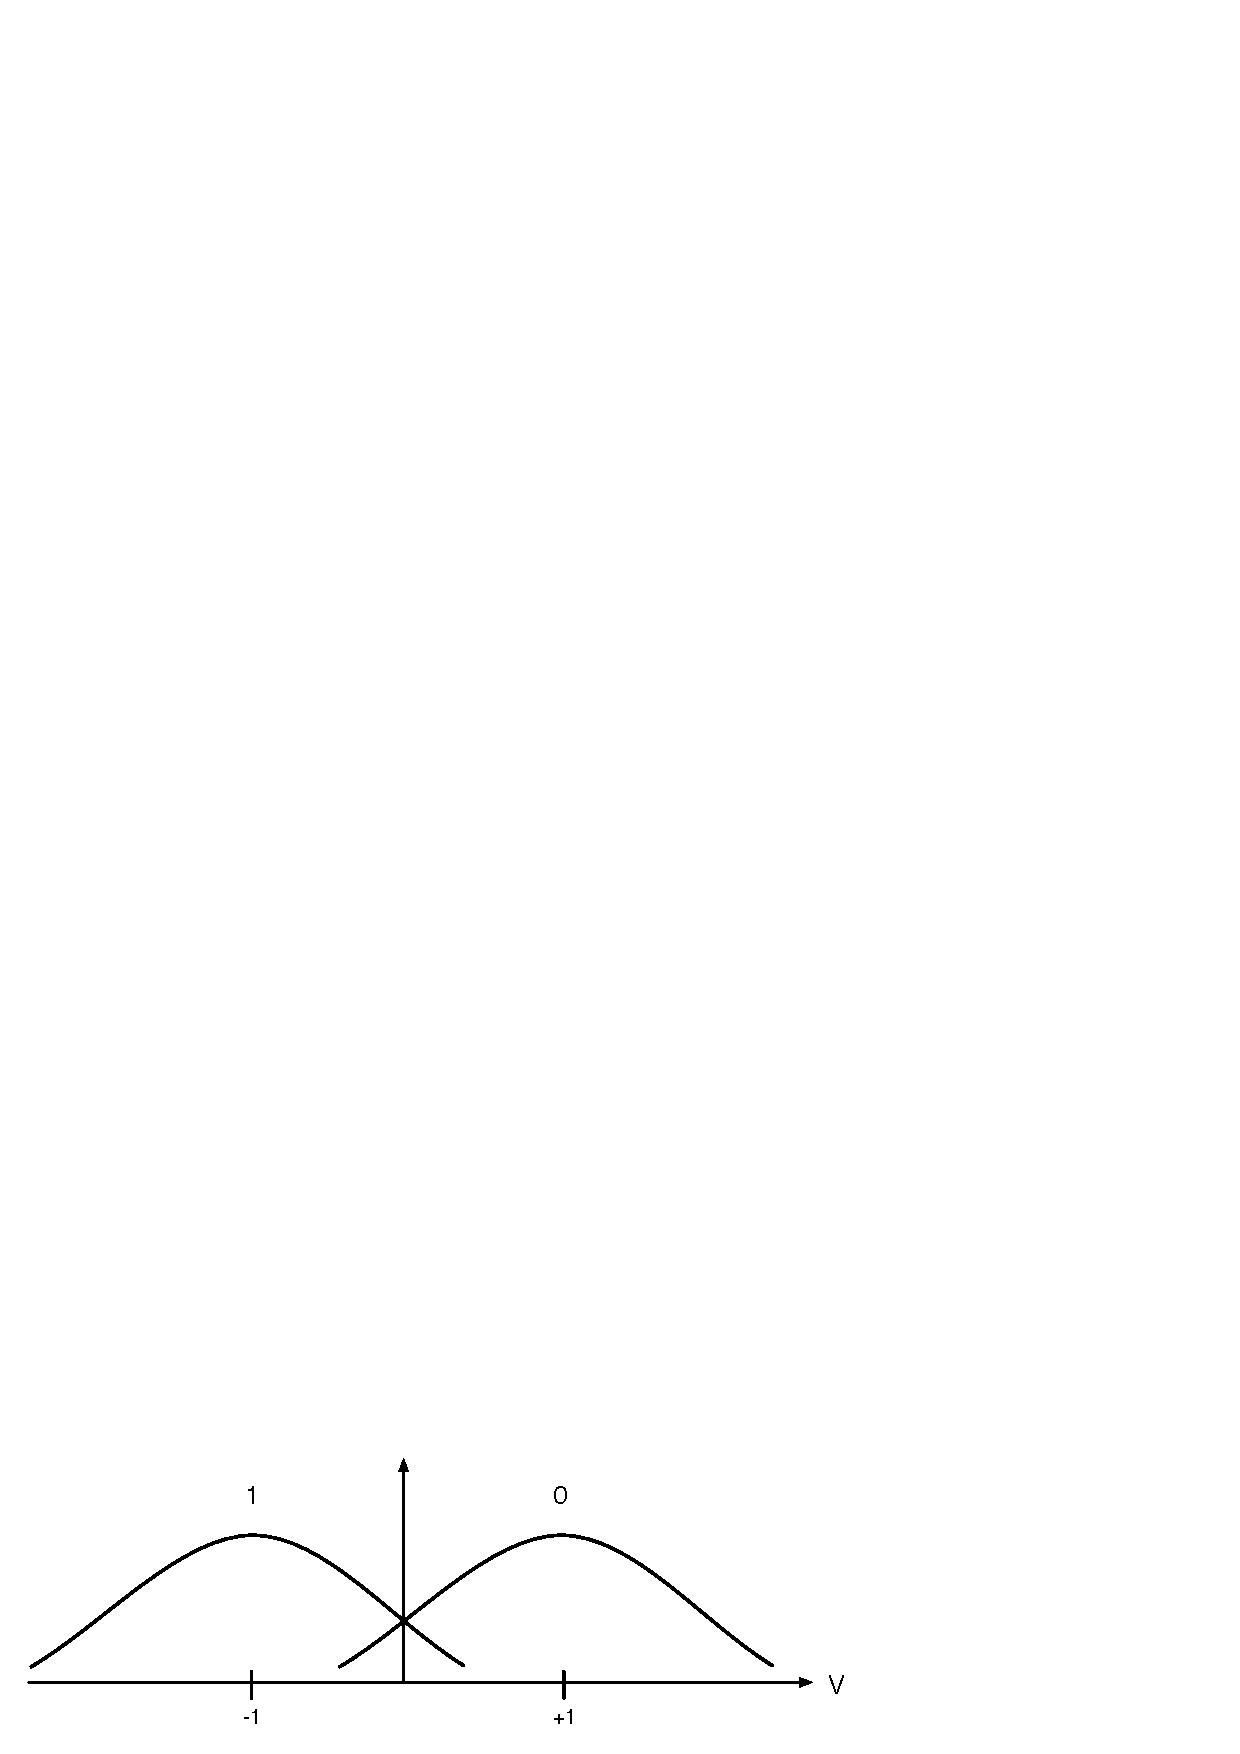
\includegraphics{BPSK_channel_graph}
\caption{Received voltage probability distribution for AWGN channel}
\label{figure:awgn probability graph}
\end{figure}

Figure \ref{figure:awgn probability graph} shows the typical probability distribution of a Binary Phase Shift Keying (BPSK) system with Additive White Gaussian Noise (AWGN). The x-axis is effectively a received voltage value from the demodulator. At transmission, a value of +1 volts corresponds to a binary 0, and a value of -1 volts corresponds to a binary 1. However, the additive noise in the channel results in the received voltage taking a range of values, and hence the received voltage is now defined as a probability distribution.

With hard decision decoding, the obvious boundary would be $x = 0$, half way between the +1 and -1 constellation symbols. Any value to the right side of this boundary would always be classified as binary 0, and anything to the left always binary 1. This means that a voltage value of 0.01 would be output as a binary 0, even though in practice it is almost equiprobable to be a binary 1. The fact that it could equally be a binary 0 or binary 1 is lost when making a hard decision, and the error correction decoder does not get that additional information.

Soft decision decoding seeks to improve on hard decision decoding, by making use of the actual received voltage value, rather than discarding it. The messages are now the conditional \textit{probabilites} of being a 1 or 0, instead of being just binary values. This allows the error correction decoder to know the degree of certainty that the message sent was a 1 or a 0.

\subsection{Hard decision decoding}
The message passing algorithm can be best understood with hard decision decoding. As an example, eq \ref{8,4 code} shows the parity check matrix $\mathbf{H}$ of an (8,4) code. This code can also be displayed, as in figure \ref{figure:tanner graph}, as a visual graph representation known as a tanner graph. [Reference: LDPC Leiner tutorial]

\begin{equation} \label{8,4 code} 
\mathbf{H} = 
\left(
\begin{array}{cccccccc}
  0 & 1 & 0 & 1 & 1 & 0 & 0 & 1 \\
  1 & 1 & 1 & 0 & 0 & 1 & 0 & 0 \\
  0 & 0 & 1 & 0 & 0 & 1 & 1 & 1 \\
  1 & 0 & 0 & 1 & 1 & 0 & 1 & 0 \\
\end{array}
\right)
\end{equation}

\begin{figure}[h]
\centering
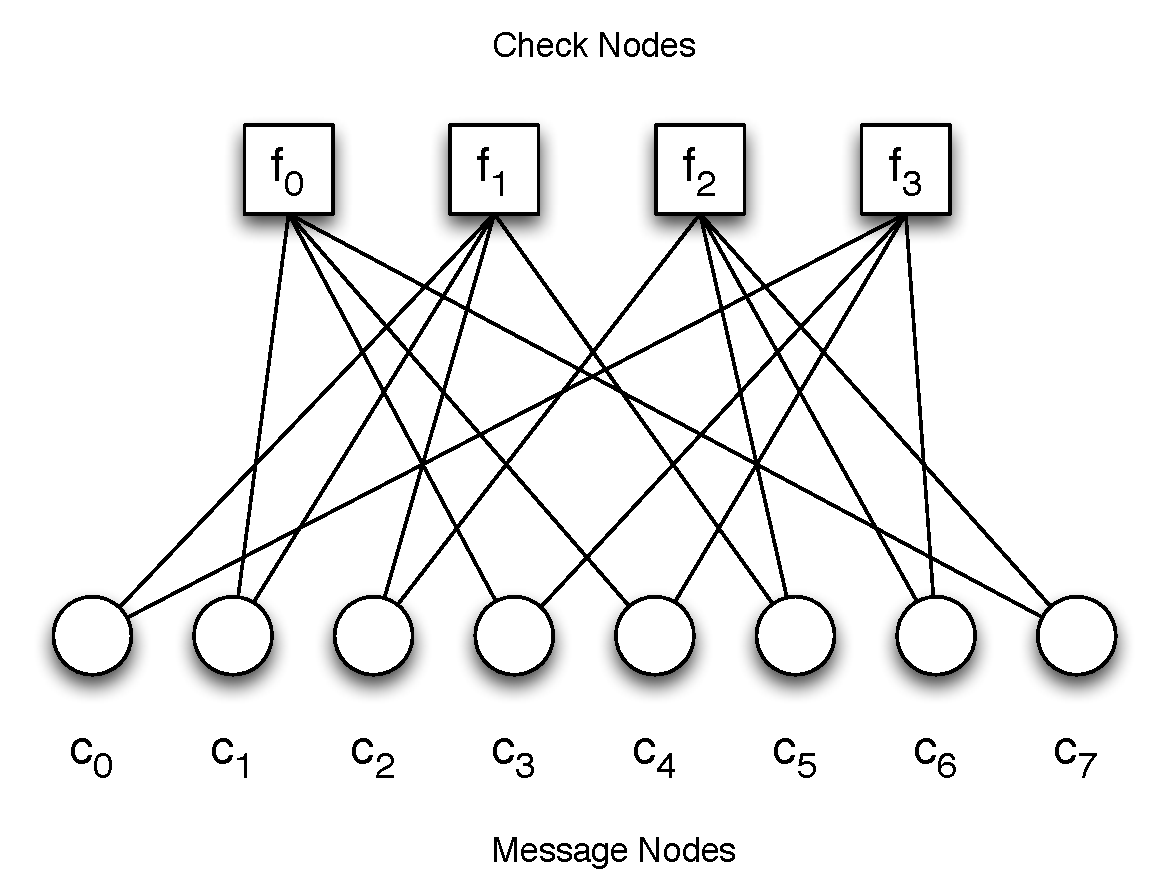
\includegraphics[scale=0.6]{tannergraph}
\caption{Tanner Graph}
\label{figure:tanner graph}
\end{figure}

The tanner graph is a bipartite graph with 2 types of node: Check nodes and Message nodes. The check nodes represent the $(n-k)$ parity check equations, whilst the message nodes represent the $n$ codeword bits. It is directly related to $\mathbf{H}$: Check node $f_j$ connects to message node $c_i$ if element $h_{ji}$ is $1$. Using the tanner graph, the hard decision decoding algorithm can now be explained as follows:
\begin{enumerate}
\item All message nodes $c_i$, having been initialised to the received codeword $y$, send their value to their connected check nodes $f_j$.
\item Each check node $f_j$ calculates a separate reply back to each message node $c_i$, with the binary value that it believes the message node should be. The parity check equation at each check node must satisfy $\lvert \sum f_j \rvert_{mod2} = 0$. From the example, check node $f_0$ receives values from $c_{1,3,4,7}$. When sending it's reply back to variable node $c_1$, it uses the values from nodes 3, 4 \& 7 along with the parity check constraint, to calculate the outbound message. Note that it does not use the information received from $c_1$ to send a reply back to $c_1$. This process continues: At each check node, a separate reply is calculated back to each connected message node.
\item The check nodes send their update back to the message nodes. Each message node in this example is connected to 2 check nodes, as well as having a previous value from step 1. As such, majority logic (with 3 bits in this case) can be used to decide whether the message node should be a 1 or a 0. 
\item The process now loops until the parity check constraint is satisfied for all nodes, at which the process terminates.
\end{enumerate}

\noindent A simple example describing the check node stage:
\begin{itemize}
\item Check node $f_0$ might receive values from $c_1$,$c_3$,$c_4$,$c_7$ = \{1,1,0,1\}.
\item To calculate the reply message to each $c_j$, use the parity check constraint $\lvert \sum f_0 \rvert_{mod2} = 0$:
\begin{itemize}
\item Reply for $c_1 : x + 1 + 0 + 1 = 0 \therefore c_1 = 0$ 
\item Reply for $c_3 : 1 + x + 0 + 1 = 0 \therefore c_3 = 0$ 
\item Reply for $c_4 : 1 + 1 + x + 1 = 0 \therefore c_4 = 1$ 
\item Reply for $c_7 : 1 + 1 + 0 + x = 0 \therefore c_7 = 0$
\end{itemize}
\item Repeat this process at all other check nodes $f_{1,2,3}$
\end{itemize}

\subsection{The Log-likelihood ratio}
Whilst hard decision decoding is a good way to demonstrate how the iterative message passing algorithm works, soft decision decoding yields substantially better error correction performance, and is therefore the main method used in decoding LDPC.

In soft decision decoding, the message nodes no longer represent binary 1's or 0's, but instead can take a continuous range of probability values. These probability values are initially calculated using two sources of information: The received voltage value of each bit, and the underlying probability distribution of the received bit. Before being able to describe the soft decision decoding algorithm, this information needs to be formed into a useful metric: the \textit{Log-likelihood ratio}, [Reference: LLR computation.pdf]

\begin{equation} \label{eq:LLR}
\mathcal{L}(c|y) = log_e \left[ \dfrac{f(c=+1|y)}{f(c=-1|y)} \right]
\end{equation}

\noindent The term $\mathcal{L}(c|y)$ is the likelihood of $c$ being transmitted given that $y$ was received. The log-ratio is able to tell us if $c=+1$ or $c=-1$ was the most likely transmitted symbol, given the received value $y$. A positive LLR indicates it is more likely that $c=+1$ was transmitted, and a negative LLR that $c=-1$ was transmitted. Additionally, the LLR has a range of $-\infty$ to $+\infty$, which provides the degree of certainty of a given symbol.

To make use of the LLR, it is necessary to manipulate it into a more useful form. Using Bayes' rule\footnote{$P(A|B) = \dfrac{P(B|A) P(A)}{P(B)}$}, and the assumption that the transmitted bits are equiprobable\footnote{i.e. $f(c=+1) = f(c=-1)$},

\begin{equation}
\begin{aligned}
\mathcal{L}(c|y) &= log_e \left[ \dfrac{f(y|c=+1) \dfrac{f(c=+1)}{f(y)}}{f(y|c=-1) \dfrac{f(c=-1)}{f(y)}} \right] 
\\
&= log_e \left[ \dfrac{f(y|c=+1)} {f(y|c=-1)} \right] 
\\
&\sim log_e \left[ \dfrac{\text{\textit{``Probability density function of +1"}}}{\text{\textit{``Probability density function of -1"}}} \right]
\end{aligned}
\end{equation}

\noindent The LLR can now be calculated for each received value of $y$. Note that it is necessary to have the underlying density functions of the received symbols. By inserting the received value $y$ into each PDF, you obtain a numerical probability of $y$ representing either +1 or -1. The ratio of these 2 probabilities then gives us the likelihood ratio.

The LLR method applies in general to all noisy channels, that is, the probability density functions can take any form. However when dealing with the AWGN channel, converting from a received symbol amplitude $y$ into the LLR is much simpler, since the probability density function in both cases is a gaussian,

\begin{equation} \label{eq:LLR_awgn}
\begin{aligned}
\mathcal{L}(c|y) &= log_e \left[ \dfrac{\mathcal{N}(1,\sigma^2)} {\mathcal{N}(-1,\sigma^2)} \right] 
\\
&= log_e \left[ \dfrac{e^{-(y-1)^2/(2\sigma^2)}}{e^{-(y+1)^2/(2\sigma^2)}} \right]
\\
&= log_e \left[ e^{4y/(2\sigma^2)} \right]
\\
&= \dfrac{2y}{\sigma^2}
\end{aligned}
\end{equation}

\noindent This result makes it very easy to take the output from the demodulator (the +1/-1 BPSK $y$ symbols) and generate the appropriate LLR's for the AWGN channel.

\subsection{Soft decision decoding}
The Belief Propagation algorithm for soft decision decoding follows a similar process to that of hard decision decoding. Messages are passed between check and variable nodes defined by the tanner graph. The main difference is what happens at each of the nodes, since now the messages are LLR's rather than binary bits. 

[Papers such as ??, ?? and ??] have all proved the set of equations that are used at both the message nodes and check nodes. The belief propagation algorithm can be distilled into just 2 equations: The message node update equation, and the check node update equation. The reason why it is often called the 'Sum-Product' algorithm, is since the message node update equation involves summing the LLR's, and the check node update equation involves taking their product.

\begin{equation} \label{eq:msgNode}
m_{ij}^{(l)} = L_i+\sum\limits_{j'\in C_i \ne j}m_{j'i}^{(l-1)}
\end{equation}

Equation \ref{eq:msgNode} is the message node update equation. $m_{ij}^{(l)}$ is the message sent from message node $i$ to check node $j$, at iteration $l$. $L_i$ is the initial LLR for message bit $i$. The expression $j'\in C_i \ne j$ is used to sum the incoming messages from all check nodes $j'$ that are connected to $C_i$, except the current node $j$ that is being sent to. This exclusion is the same as for hard decision decoding, whereby a message to a node is never a function of a message from that node (the extrinsic information rule). Finally, $m_{j'i}^{(l-1)}$ indicates that the sum is of the received check node messages from the last ($l-1$) iteration.

\begin{equation} \label{eq:chkNode}
m_{ji}^{(l)} = 2\arctanh\left[\prod\limits_{i'\in V_j\ne i} \tanh(\dfrac{m_{i'j}^{(l-1)}}{2})\right]
\end{equation}

Equation \ref{eq:chkNode} is the check node update equation. $m_{ji}^{(l)}$ is the message sent from check node $j$ to message node $i$, at iteration $l$. As before, $i'\in V_j\ne i$ includes all message nodes $i'$ that are connected to check node $V_j$, except the current node $i$ that is being sent to (extrinsic information rule).

\noindent With both node equations defined, the iterative soft decision decoder proceeds as follows:

\begin{enumerate}
\item All message nodes $c_i$, having been initialised to the received LLR's $L_i$, send their value to their connected check nodes $f_j$. 
\item At each check node $j$, using equation \ref{eq:chkNode}, the return message to each connected message node $i$ can be calculated.
\item Sum the LLR's received at each message node, and obtain the binary value of the codeword ($l_i > 0 \rightarrow 0$, $l_i < 0 \rightarrow 1$). Using the parity check equation $\mathbf{s=c H}^\top$, where $c$ is the current binary value of the codeword, we obtain the syndrome. If the syndrome is all-zero, the algorithm terminates, since a valid (though not necessarily correct) codeword $c$ has been found.
\item At each message node $i$, using equation \ref{eq:msgNode}, the return message to each connected check node $j$ can be calculated.
\item Steps 2-4 repeat until a valid codeword is found, or up to a maximum number of iterations (Usually around $l=50$). 
\end{enumerate}

\subsection{Min-Sum approximation}

Min sum to go in here

\section{The AWGN channel: Simulation \& Results}
One of the most important noisy channels used in communications theory, and already mentioned previously, is the Additive White Gaussian Noise (AWGN) channel. Whilst this noise channel is not really applicable to model Flash Memory, which is the aim of this project, it is however a useful benchmarking tool to ensure that the MATLAB decoder is working correctly. It is also a good method of demonstrating the power of LDPC, soft decision decoding, and error-correcting codes generally. This section presents the work done in modelling the encoder, AWGN channel, and decoder, and compares the results to known data sets.

\subsection{Simulation model}
\begin{figure}[h]
\centering
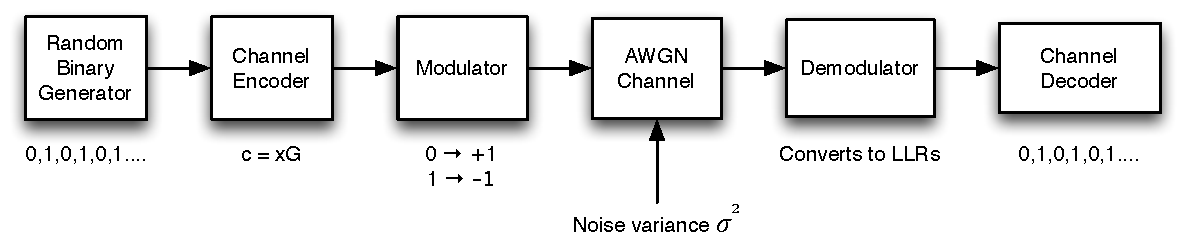
\includegraphics[scale=0.878]{awgn_channel_model}
\caption{The AWGN simulation model}
\label{figure:awgn sim model}
\end{figure}

\begin{itemize}
\item The random generator produces a vector of pseudo-random, uniformly distributed values from the set \{1,0\}, of length $k$.
\item The channel encoder takes the length $k$ message, and encodes it using the generator matrix, into a block of length $n$.
\item The modulator maps each binary bit, in this case using Binary Phase-Shift Keying (BPSK), onto a constellation symbol. These symbols represent a real voltage value.
\item The channel is simulated by adding white gaussian noise onto each symbol. The output from the channel is $\mathbf{Y = X + N}$, where $\mathbf{X}$ is the input random variable (+/- 1), and $\mathbf{N}$ is the noise random variable ($\mathbf{N} \sim \mathcal{N}(0,\sigma^2)$)
\item The demodulator, for soft decision decoding, calculates the LLR of each received symbol. From equation \ref{eq:LLR_awgn}, $\mathcal{L} = \dfrac{2y}{\sigma^2}$, where $y$ is the received value from the output of the channel, and $\sigma^2$ is the AWGN channel noise variance. In a real system, this method therefore requires knowledge of the underlying noise parameters. For the simulation, the value is assumed to be known.
\item Finally, the channel decoder performs error correction using the Belief Propagation algorithm, and outputs the corrected codeword (Note: The encoded message can be extracted from the codeword if a systematic generator matrix was used).
\end{itemize}

To simulate the error correction performance of this system, and compare it to other results, there needs to be a standardised quantity to describe the error rate and the channel noise. Whilst the noise variance is one such quantity, it doesn't take into account the relative difference between signal power and noise power. A far more useful metric would be Signal-to-noise ratio (SNR), or more specifically in this case $\dfrac{E_b}{N_0}$ (energy per bit/noise power). Like SNR, this is usually given in decibels\footnote{For the conversion calculations, $\dfrac{E_b}{N_0}$ must be a linear, not logarithmic, value. i.e: $\dfrac{E_b}{N_0}(\text{dB}) = 10\log_{10}\left[\dfrac{E_b}{N_0}(\text{lin})\right]$}. 
\vspace{3mm} \\
\noindent
Converting between $\sigma^2$ and $\dfrac{E_b}{N_0}$ is relatively trivial:
\vspace{3mm} \\
\noindent
\begin{tabular}{lcl}
$E_s$ & - & Energy per symbol (Always 1 for BPSK) \\
$R_c$ & - & Code rate \\
$R_m$ & - & Modulation rate (Always 1 for BPSK) \\
$E_b$ & - & Energy per information bit \\
\end{tabular}
\begin{equation} \label{eq:noisePwr}
\sigma^2 = \dfrac{N_0}{2}
\end{equation}
\begin{equation}\label{eq:EnergyperSymbol}
E_s = R_cR_mE_b
\end{equation}
$N_0$, the noise power, is defined as in \ref{eq:noisePwr}. The energy per symbol is defined in \ref{eq:EnergyperSymbol}: the energy per bit multiplied by both the number of bits per symbol and the ratio of useful message data. By substituting $E_s$ into $\dfrac{E_b}{N_0}$:
\begin{equation}
\begin{aligned}
\dfrac{E_b}{N_0} &= \dfrac{E_s}{R_cR_mN_0} \\
&= \dfrac{E_s}{R_cR_m2\sigma^2} \\
&= \dfrac{1}{2R_c\sigma^2}
\end{aligned}
\end{equation}
$E_s = R_m = 1$ in this case, further simplifying the equation. This allows the conversion between $\sigma^2$, the parameter used in the noise model, and $\dfrac{E_b}{N_0}$, the metric used to present the results.

The dependent variable in the simulation is the Bit Error Rate (BER). The output from the channel encoder is compared to the output from the channel decoder, where both are blocks of length $n$. The number of bit errors is simply the difference between the two codewords (similar to the Hamming distance). This raw bit error number is then divided by the block length, to obtain a bit error rate.

Each instance of the block diagram in figure \ref{figure:awgn sim model} generates a random binary block, and the noise added to that block is also random. A single sample will not be sufficient to get an accurate error rate of the system for a given noise value, since at very low error rates thousands of blocks may need to be decoded before a single bit error occurs. Performing a simulation of repeated sampling is known as a Monte Carlo simulation. The process in MATLAB is therefore designed to perform $N$ trials of the simulation, with each trial outputting a bit error rate. After completing all trials, the bit error rate can be averaged over all blocks. In this project, for the lowest bit error rate experiments, up to $10^6$ blocks were processed per noise value.

\subsection{Simulation results}
\begin{figure}[h]
\centering
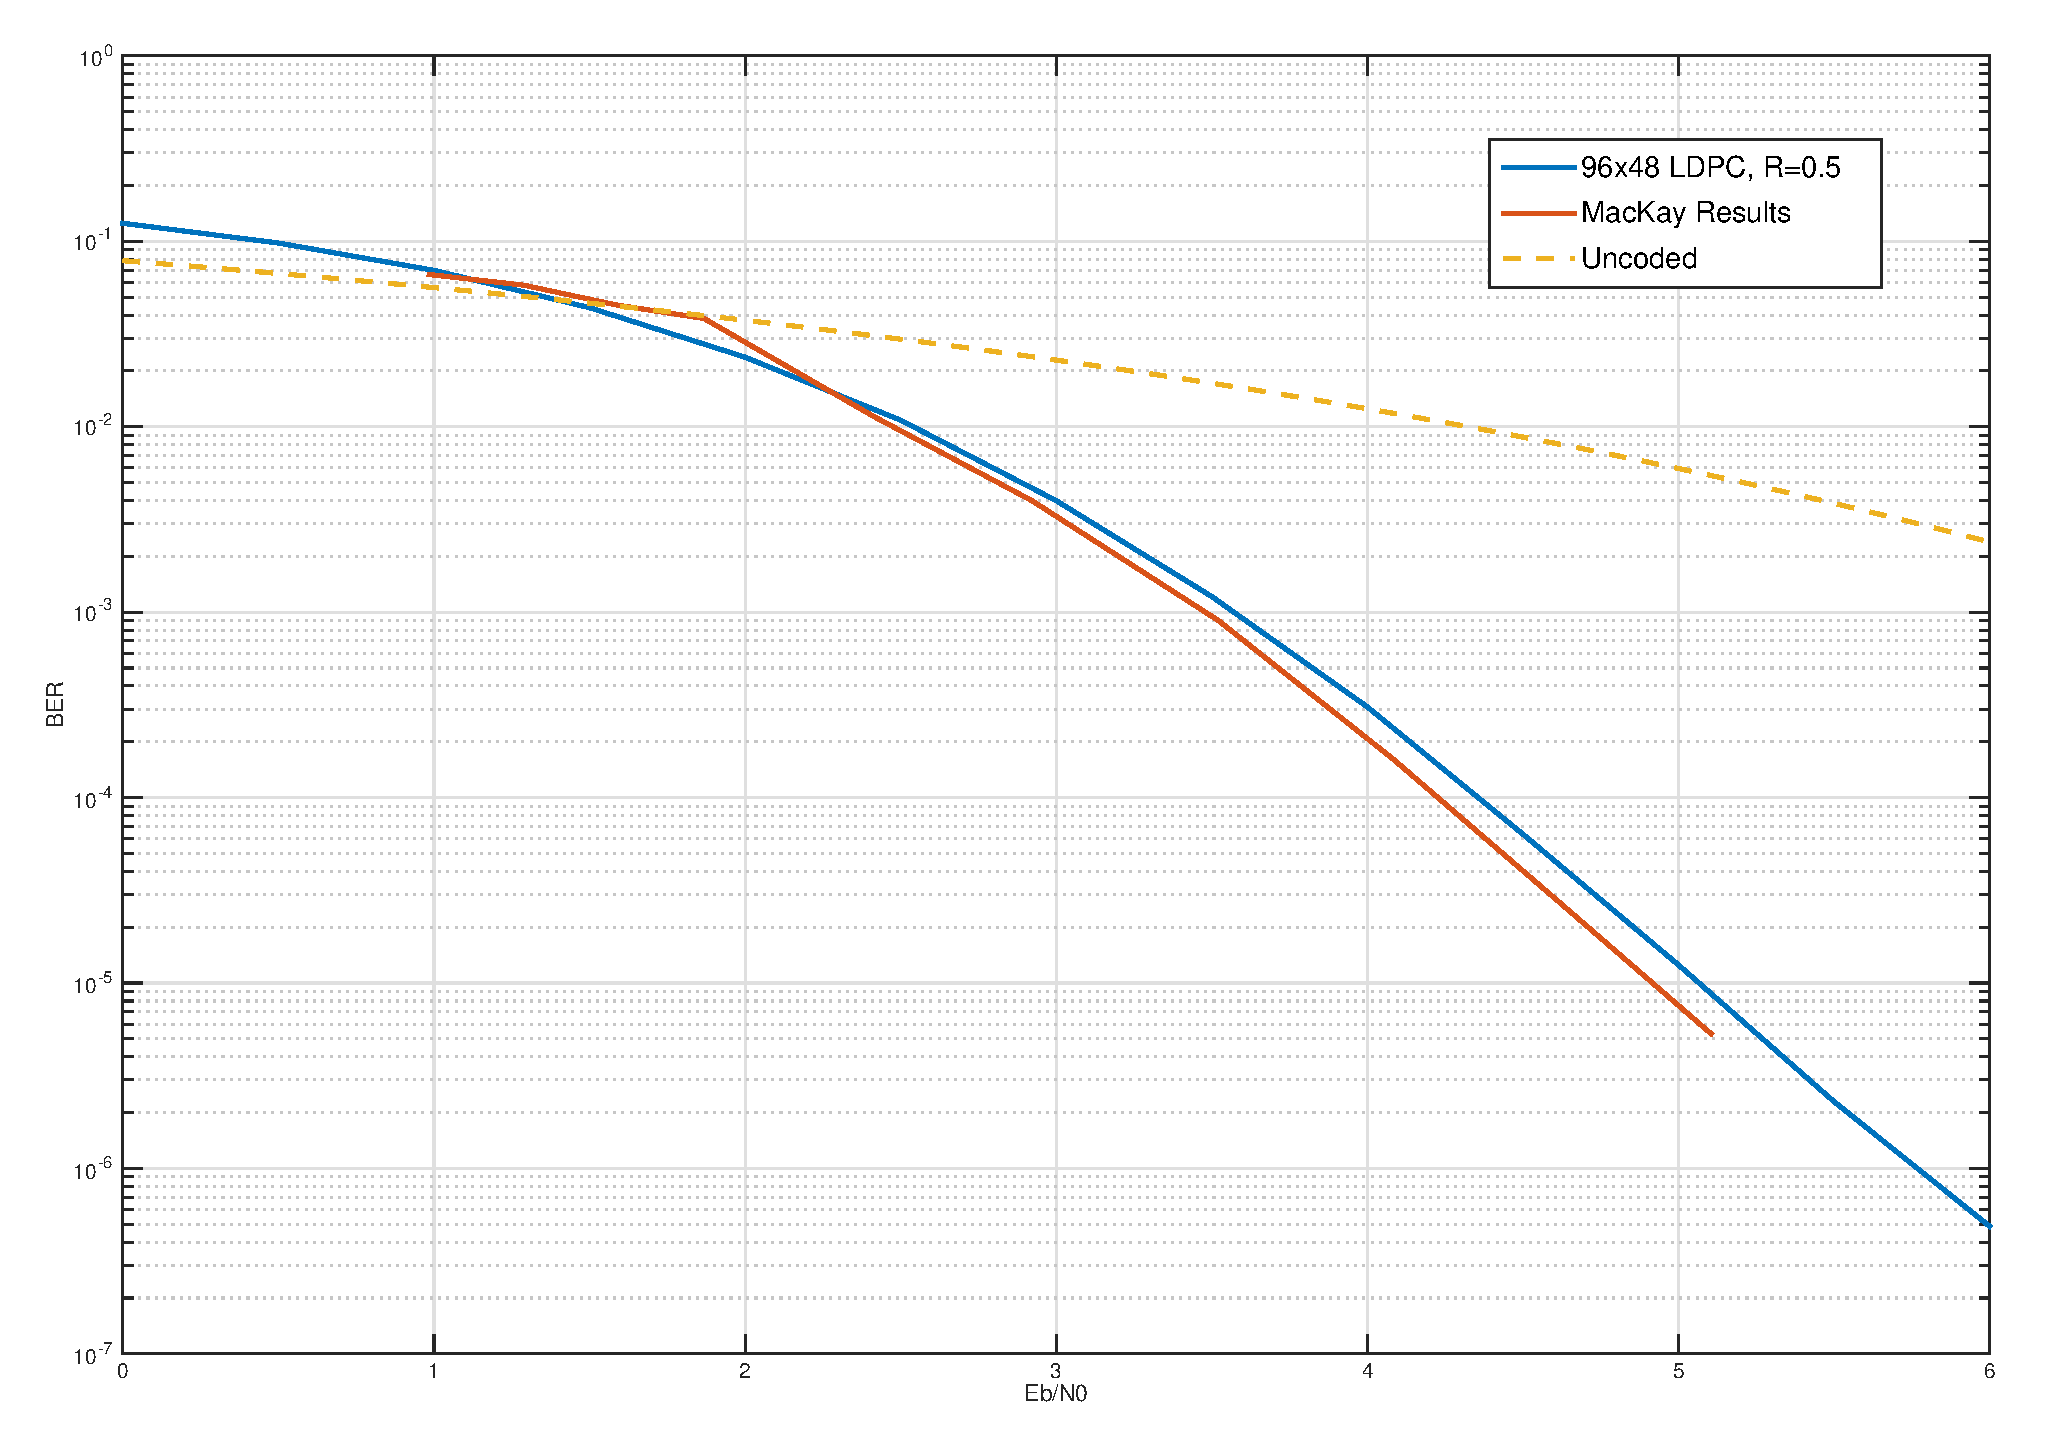
\includegraphics[scale=0.5]{96_48_LDPC}
\caption{Simulated results of 96,48 LDPC code}
\label{figure:96_48_LDPC_graph}
\end{figure}

A short block length, rate $\dfrac{1}{2}$ LDPC code was used to produce the results in figure \ref{figure:96_48_LDPC_graph}, using the Sum-Product algorithm with soft decision decoding. The figure also displays the results obtained by MacKay using the same LDPC code and decoding method. There is a minor performance loss compared to MacKay, but otherwise the results are in agreement. Additionally, the dashed line indicates the expected bit error rate in the event that no error correction code was used. There is therefore a substantial coding gain in this system, for example to achieve a BER of $10^{-6}$ requires around $5.5$ dB with coding, and nearly $10$ dB without.

\begin{figure}[h]
\centering
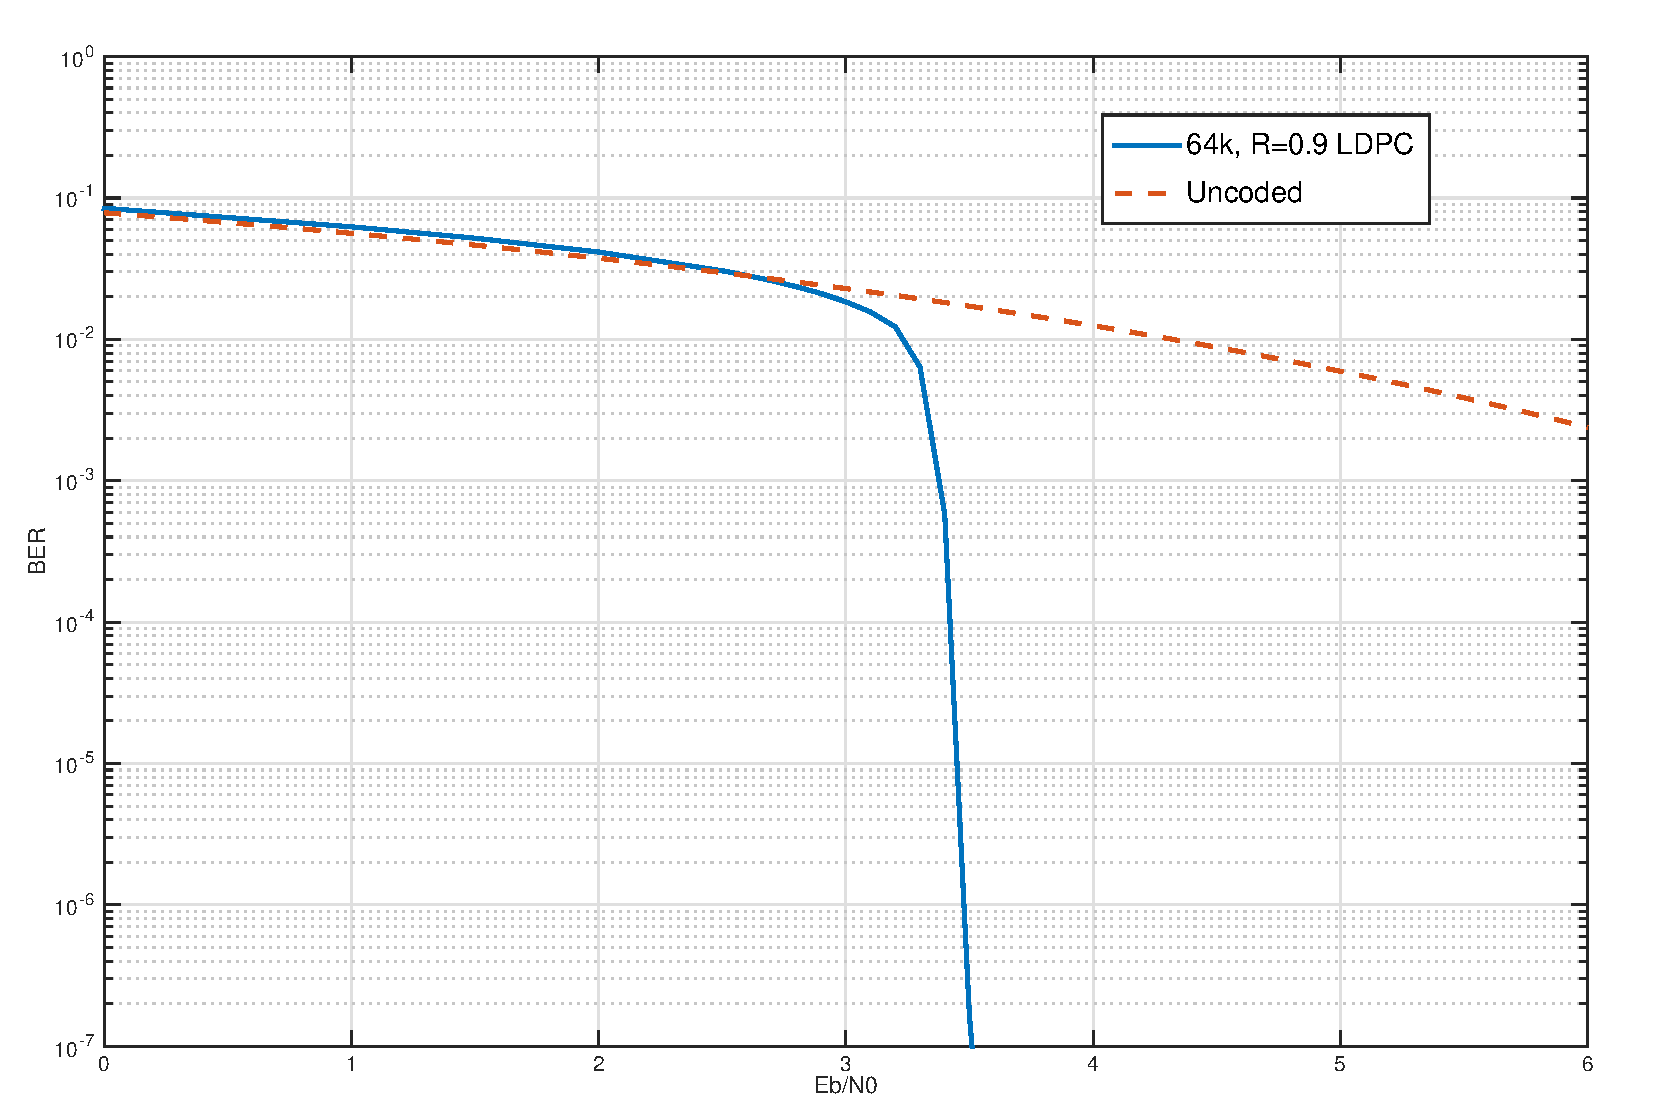
\includegraphics[scale=0.6]{dvbs2_graph}
\caption{Simulated results of 64k DVB-S2 LDPC code}
\label{figure:64k_LDPC_graph}
\end{figure}

Longer block length codes generally achieve superior performance and greater 'cut-off' compared to shorter codes. Figure \ref{figure:64k_LDPC_graph} demonstrates a code with a block length of $64000$, and a substantially higher rate ($R=0.9$). This particular code is a standardised construction, used in the DVB-S2 (Satellite broadcasting) specifications. This code is also the primary one used in this project for the memory error correction later. One benefit of using this code is its sharp 'cut-off', compared to the previous code in figure \ref{figure:96_48_LDPC_graph}.

\subsection{Conclusion}
Simulating the AWGN channel, and then comparing the results to the known data published by MacKay, allows for some degree of verification of the MATLAB program. The AWGN channel is one of the common channels simulated when dealing with error correcting code, since it simulates the effect of random noise that often occurs in the environment. 

One issue identified with the simulation program was the speed of the decoder. In the first version of the decoder program [?? Matlab appendix section], there were a substantial number of 'for' loops, which are generally slow in MATLAB. Subsequent versions of the decoder attempted to fix this by vectorising the code [?? Matlab appendix section 2], resulting in a ???x speed increase. However, even with these improvements, the decoder was still much slower compared to MATLAB's built-in LDPC decoder [?? matlab reference page]. In addition, freely available OpenCL accelerated decoders [?? openCL ref] can be used on a GPU (Graphics Processing Unit) which are even faster than MATLAB's implementation (See appendix [??] for the benchmark comparisons). In the subsequent sections simulating the memory model, the MATLAB built-in implementation of the LDPC decoder was used, allowing for substantially more blocks to be decoded in the same amount of time.

\section{Modelling a memory-specific noise channel}
There are many similarities between modelling a communications system and flash memory. Both are binary channels, subject to some binary input, distortion by some noise source, and subsequent decoding. However, the major difference in flash memory is the storage of binary data in the device for a length of time, unlike a communications system where the data is 'in transit'. When a bit is stored to a memory cell, the noise effect is cumulative over the lifetime of the stored bit. Therefore, two major parameters in modelling flash memory are time, and the number of read/write (or Program/Erase) cycles each cell is subject to.

As stated previously in section [??], it is the threshold voltage of each gate that defines the binary value of the memory cell. In this project, the flash memory is assumed to be of SLC design, that is 1 bit per cell. It is also assumed that a low gate threshold voltage corresponds to a binary 0, whilst a higher threshold voltage corresponds to a binary 1. 

The primary noise source, which is caused by repeated P/E cycling, can be split into two physical phenomena: Electron capture and emission events, which result in a random variation of the threshold voltage, and interface trap recovery and electron de-trapping, which gradually reduces the gate threshold voltage over time. The former is known as `Random Telegraph Noise' (RTN), whilst the latter is often called the `Retention Noise', since it sets a time limit on how long data can be stored in a cell until the threshold voltage becomes too low.

Another noise source, known as `Cell-to-cell interference', which as the name implies is the result of neighbouring memory cells interfering with each other. This dependence between neighbouring cells adds additional complexity when modelling the system, since it is no longer possible to model one cell at a time. As a result, it was decided for this project not to include this noise source, instead focusing on an individual memory cell.

\subsection{Description of Noise Sources}

The first noise source in the memory channel, the random telegraph noise (RTN), can be modelled as a Laplacian distribution, $Y_{rtn} \sim \mathcal{L}(\lambda_{rtn})$, whose probability density function is
\begin{equation} \label{eq:RTN}
p_{rtn}(x) = \dfrac{1}{2\lambda_{rtn}}e^{-\lvert x \rvert / \lambda_{rtn}}
\end{equation}
In equation \ref{eq:RTN}, $x$ is the value of the voltage fluctuation, and $\lambda_{rtn}$ scales with $N$, the P/E cycling number. In this project, $\lambda_{rtn} = K \sqrt{N}$ where $K$ is just a constant. Therefore as the memory cell is subject to more P/E cycles ($N$), the RTN distribution widens, as expected. Figure \ref{figure:RTN_graph} shows the probability density function of the distribution for different values of $N$. The distribution is centered about $x=0$, since the random effect of RTN can result in either an increase of decrease of the cell threshold voltage.

\begin{figure}[h]
\centering
\minipage{0.5\textwidth}
\centering
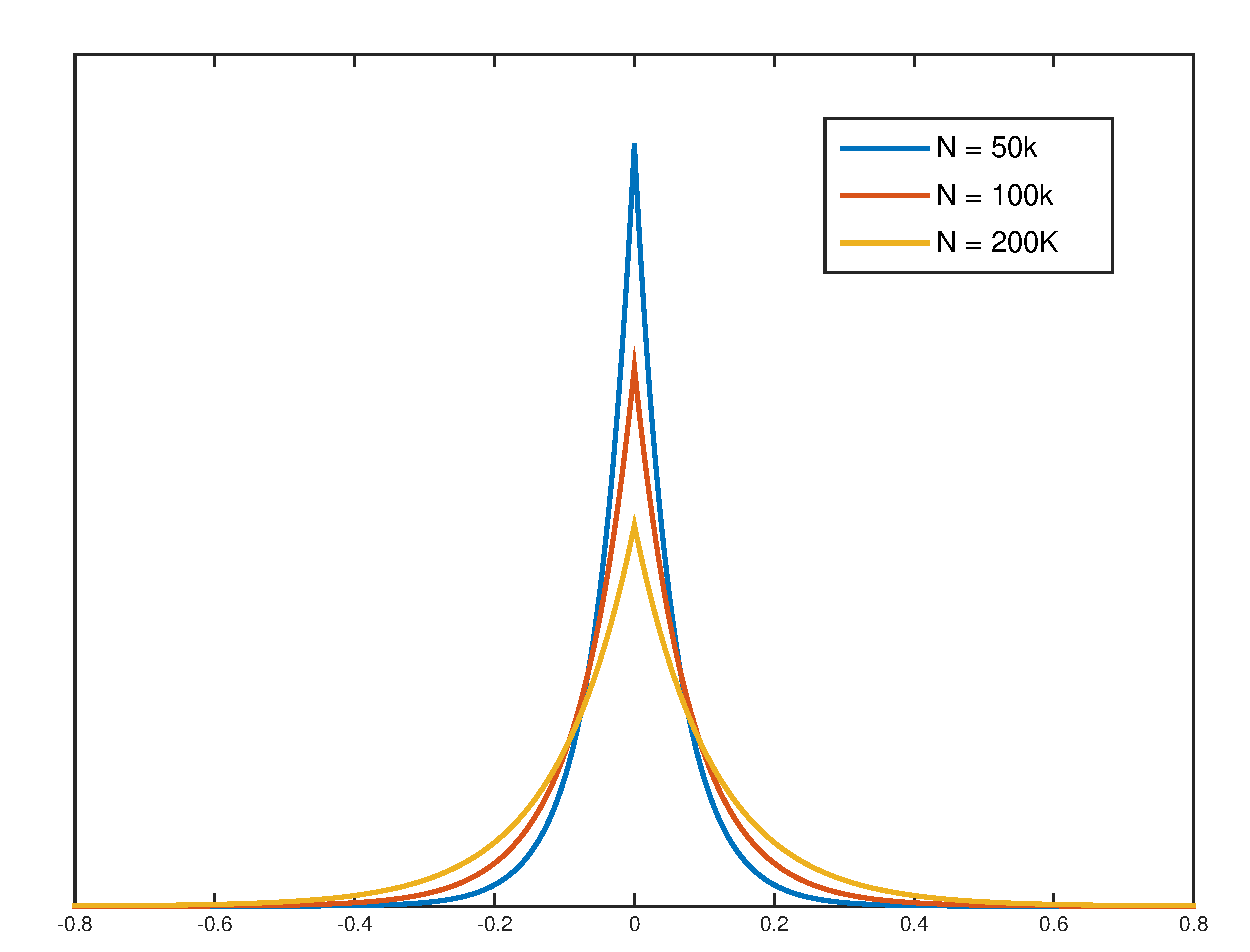
\includegraphics[scale=0.42]{RTN_graph}
\caption{PDF of RTN distribution}
\label{figure:RTN_graph}
\endminipage\hfill
\minipage{0.5\textwidth}
\centering
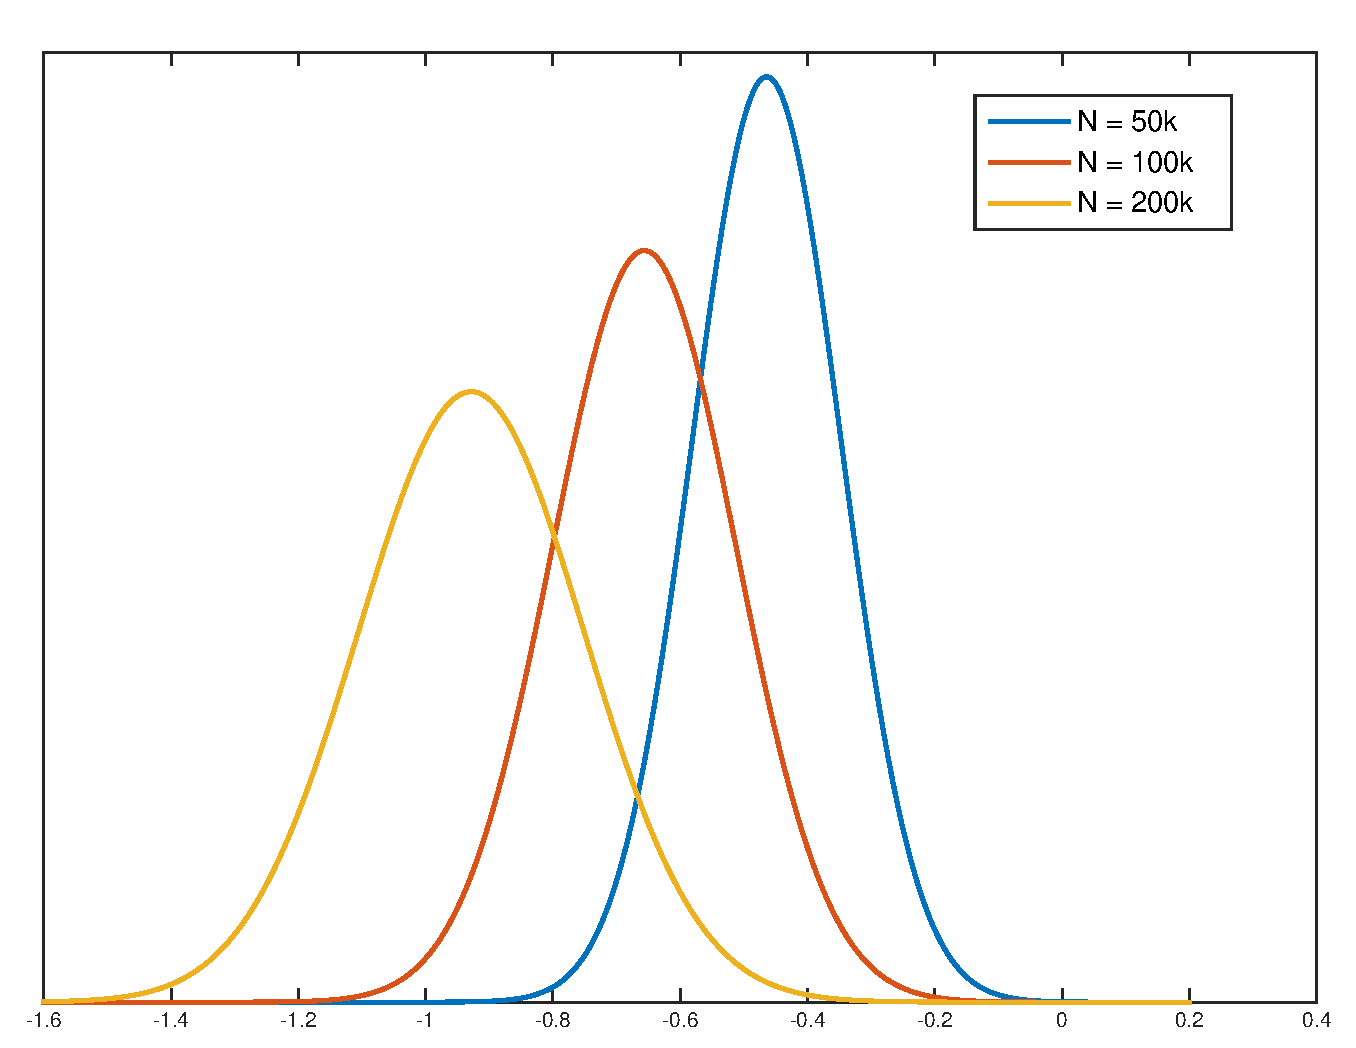
\includegraphics[scale=0.378]{retention_noise_graph}
\caption{PDF of Retention noise distribution}
\label{figure:ret_graph}
\endminipage
\end{figure}

The second noise source, the retention noise, is modelled as a Gaussian, $Y_{retention} \sim \mathcal{N}(\mu_r,\sigma_r^2)$, with the mean and variance defined as
\begin{equation} \label{eq:retention}
\begin{aligned}
\mu_r &= -K_sK_d(V_p-V_e)N^{0.5}\ln\left(1+\dfrac{t}{t_0}\right)\\
\sigma_r^2 &= K_sK_m(V_p-V_e)N^{0.6}\ln\left(1+\dfrac{t}{t_0}\right)
\end{aligned}
\end{equation}
In equation \ref{eq:retention}, $V_p$ is the initial voltage of the programmed state, $V_e$ is the (mean) voltage of the erased state, $t$ is the current memory retention time, and $t_0$ is an initial starting time. $K_{s,d,m}$ are all constants. The retention noise therefore has a power-law relationship with the P/E cycling number $N$, a logarithmic relationship with retention time, and is also dependent on the initial threshold voltages. Figure \ref{figure:ret_graph} shows the probability density function of the retention noise for different values of $N$, with the remaining variables fixed. Also note that since the mean ($\mu_r$) is always negative, the effect of the Retention noise is to always reduce the gate threshold voltage. As $N$ increases, the programmed state voltage will therefore reduce and get closer to the erased state voltage. This is perhaps the main source of bit error: the interference between the erased and programmed states. 

\subsection{Channel Model}
Both the RTN and retention noise are independent random variables. Therefore the threshold voltage of any given cell is simply the sum of the random variables. As explained previously in section [??], each cell is either a binary 0 or 1, with a corresponding threshold voltage distribution for each. Therefore in the ideal case each cell will have a single voltage value, either $V_{p_0}$ for a programmed cell or $V_{e_0}$ for an erased cell. After noise, the final threshold voltage of the cell is then

\begin{equation}
\begin{aligned}
V_{p} &= V_{p_0} + Y_{rtn} + Y_{retention} \\
V_{e} &= V_{e_0} + Y_{rtn}
\end{aligned}
\end{equation}
where $V_{p}$ and $V_{e}$ are the final programmed and erased voltage states, respectively. Retention noise is not added onto the erased state in this model, since we are assuming that the erased state is the reference voltage level that the retention noise is derived from.
\bigskip

\begin{figure}[h]
\centering
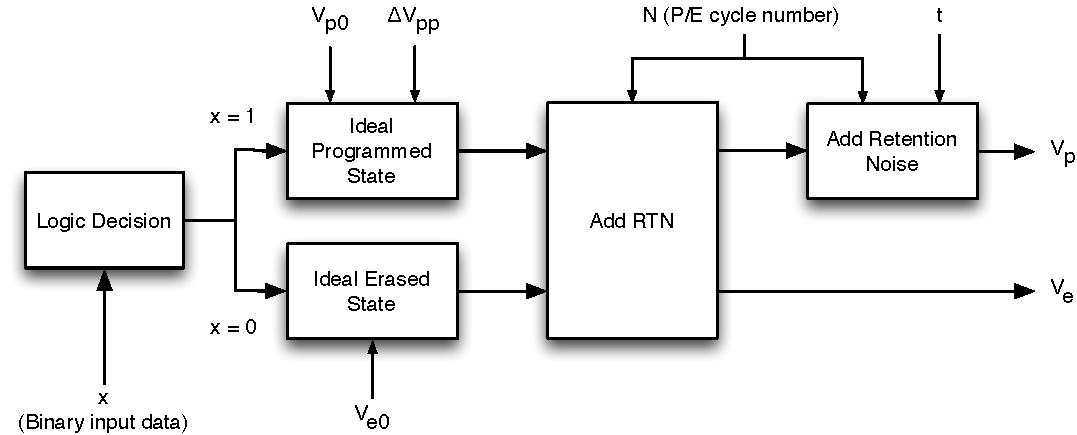
\includegraphics[scale=0.96]{memory_channel}
\caption{Memory channel noise model}
\label{fig:mem_channel_model}
\end{figure}

Figure \ref{fig:mem_channel_model} shows the block diagram of the memory channel noise model. Unlike the AWGN channel, the noise added to each binary bit depends on whether it is a 0 or a 1. The input to the model is a binary value, whilst the output from the model is the final threshold voltage value of the memory cell, ready to be decoded. Effectively, the model simulates the programming of a memory cell, and then the subsequent noise that would be experienced if the cell were subjected to repeated program and erase cycles.

\begin{figure}[!ht]
\centering
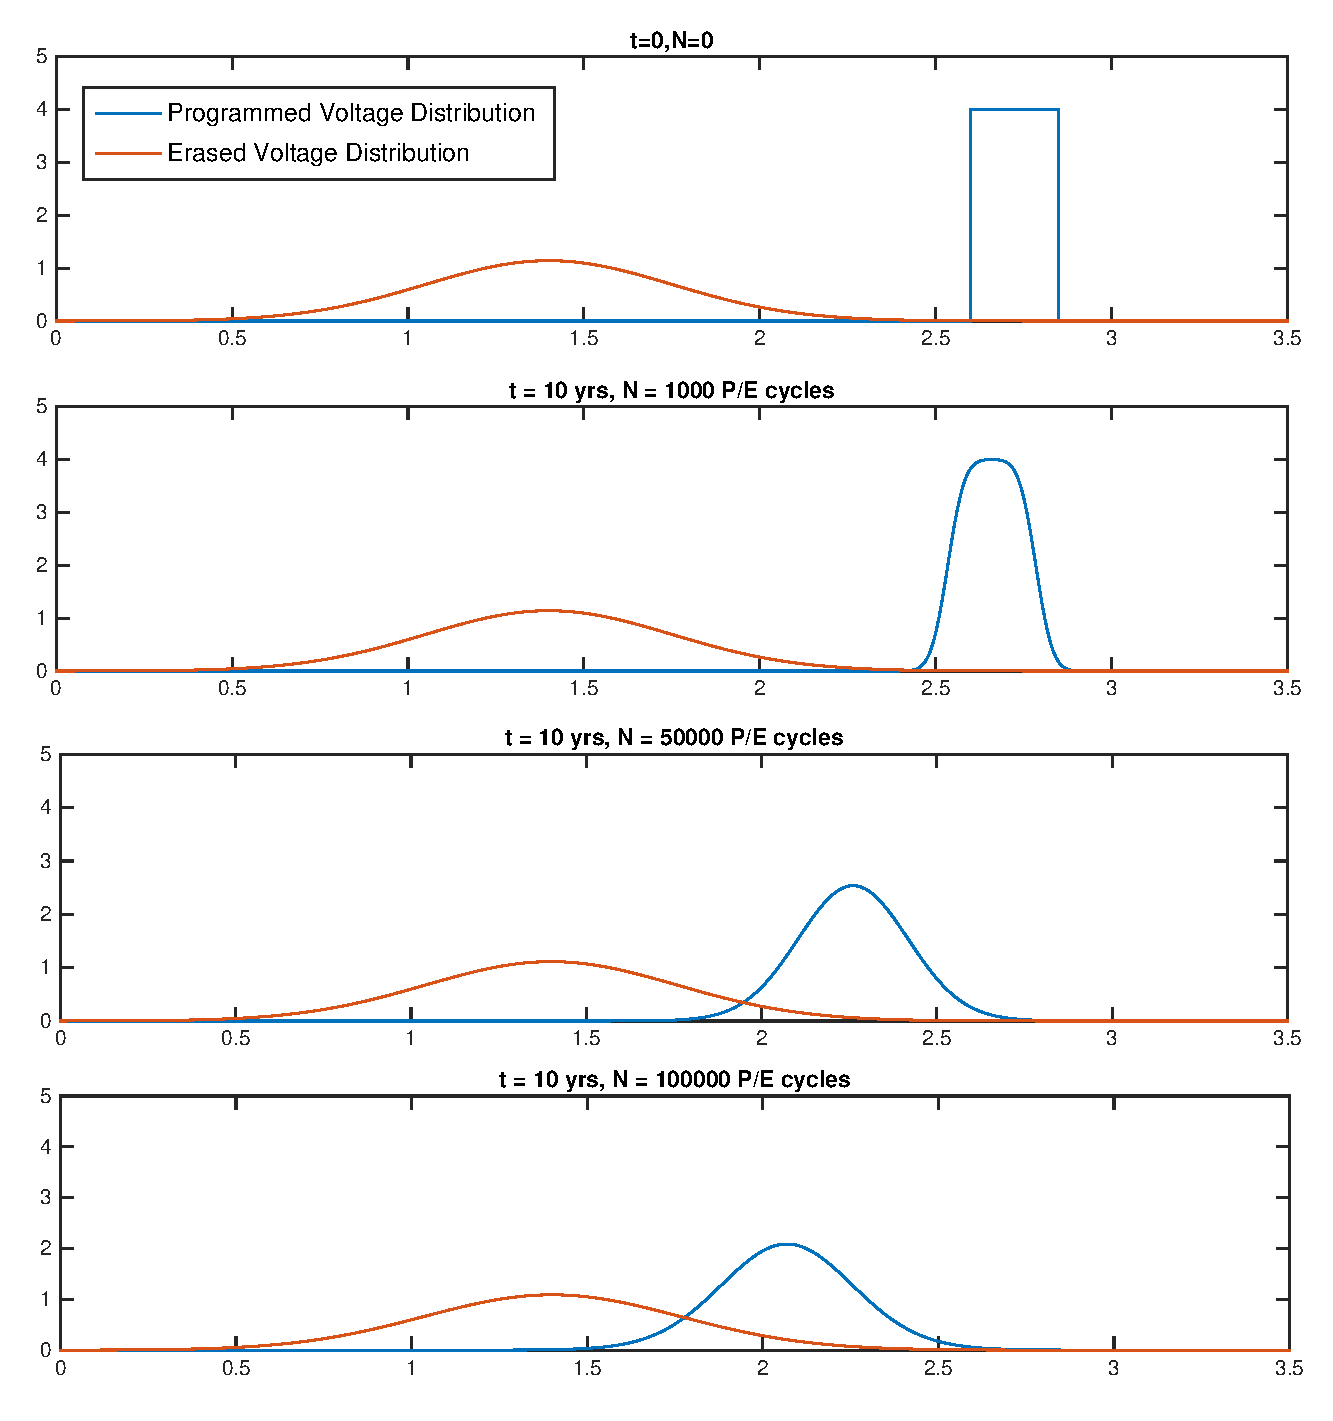
\includegraphics[scale=0.75]{memory_voltage_distribution}
\caption{Density functions of memory threshold voltages for differing values of N}
\label{fig:mem_channel_distribution}
\end{figure}

Figure \ref{fig:mem_channel_distribution} shows the probability density functions obtained from the memory model in figure \ref{fig:mem_channel_model}. Note that the $x$ axes are the gate threshold voltages. Various values for $N$ are displayed as well as showing the initial programmed state (the uniform distribution) when $N=0$. As the number of P/E cycles increases, the programmed distribution shifts left and widens, and interferes with the erased state. It is now clear that a simple hard-decision decoder without any error correction would generate a substantial number of errors when, in this case, $N > 50,000$. The distributions overlap, which would lead to incorrectly decoded bits.

\section{Decoding in the non-Gaussian case}

\section{The memory channel: Simulation \& Results}

\section{Conclusions}

\phantomsection
\addcontentsline{toc}{section}{Appendix A: Random Number Generation}
\section*{Appendix A: Random Number Generation}
When performing any sort of Monte Carlo simulation, and particularly if running the same program in parallel across multiple computers, it is important to ensure that the random numbers being generated are as random as possible. Even more crucially, there must be no dependence between the parallel task's random numbers if we are to combine result sets.

MATLAB, like many other software packages, cannot generate truly random numbers. Instead, it uses a pseudo-random number generator, such as the Mersenne Twister algorithm. This is just a function that produces numbers which, for most purposes, are considered to be pseudo-random and pseudo-independent. That is, if you generate numbers from this algorithm, they will appear to be random samples from a uniform distribution. 

However, the Mersenne Twister algorithm actually has a finite period. After generating $2^{19937}$ random numbers, the output begins to repeat itself. More importantly, every time MATLAB starts, the random generator is reset to the same position. This means if you try to generate a large set of random numbers in MATLAB, you will always get exactly the same numbers. Effectively, MATLAB uses the same \textit{seed} to the random number generator on every start-up. This is meant to be useful for debugging purposes, however when running simulations in parallel, it causes all the result to no longer be independent. This means you cannot combine results made in parallel, since the output from each parallel stream will actually be identical.

The solution is to ensure that every task executed in parallel has a random seed fed into the random number generator. Effectively, the seed is used as the starting position for the Twister algorithm. If the seed is a truly random number, then each random generator should start in a different position. Any two random generators might start with billions of positions between them, or possibly right next to each other. But the chances of an identical start position are negligible.

\begin{lstlisting}[float=ht,style=Matlab-editor,caption = {Seeding random generator},label=code:rng]
% Ensures truly random numbers for each process
% seed is now a random number that can be used to initialise rand
fid = fopen('/dev/random');
seed = fread(fid, 1, 'uint32');
RandStream.setDefaultStream(RandStream('mt19937ar','seed',seed));
\end{lstlisting}

The commands in codebox \ref{code:rng} were used to seed the random number generator every time a new MATLAB process was created. On UNIX machines, there is a system random number source \mbox{`/dev/random'}, which ``gathers environmental noise from device drivers and other sources into an entropy pool [and] from this entropy pool random numbers are created." The numbers generated by this process originate from physical random processes such as hardware noise, and so it is assumed that when calling the function on a different machine, a different random number will be generated every time. These random numbers are then used to seed the pseudo-random stream in MATLAB. 

\end{document}